\section{Auswertung}
\label{sec:auswertung}

Die aufgenommenen Messdaten werden mit Hilfe von den Python Pakten Matplotlib \cite{matplotlib} und Numpy \cite{numpy}
ausgwertet. 

\subsection{Magnetfeld}

Die aufgenommen Messwerte der magnetische Flussdichte werden in der Tabelle \ref{tab:feld} dargestellt.
Es wurde die Flussdichte $B$ an der jeweiligen Position $z$ notiert.
Die Reihenfolge in der die Werte dargestellt sind entspricht auch der Reihenfolge in der die Messwerte aufgenommen wurden.
Dabei wurde die Mitte in dem Lufspalt per Auge abgeschätzt.

\begin{table}[H]
	\centering
	\caption{}
	\input{build/table_field.tex}
	\label{tab:feld}
\end{table}

Zur Bestimmung der maximalen Flussdichte werden die in der Tabelle \ref{tab:feld} angegebenen Werte in dem 
Plot \ref{fig:feld} aufgetragen.

\begin{figure}[H]
    \centering
    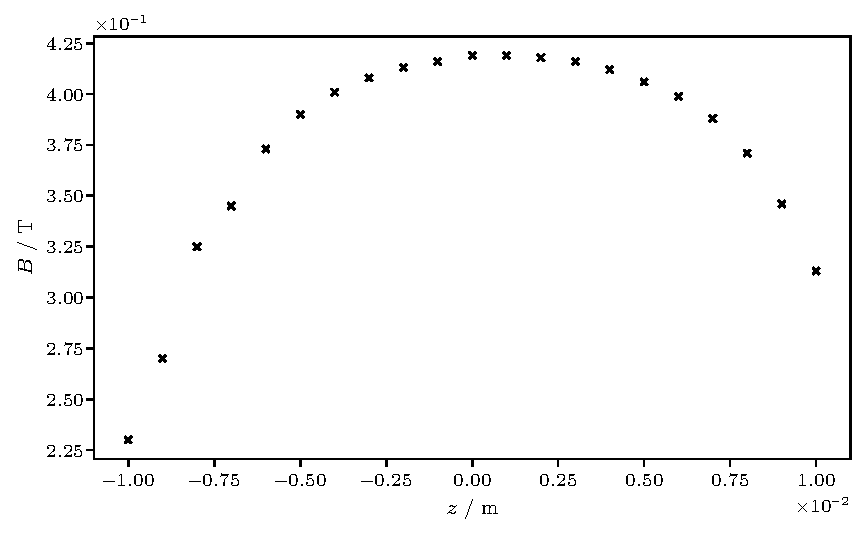
\includegraphics{build/field.pdf}
    \caption{Messung zum Verlauf des Magnetfeldes um den Luftspalt.}
    \label{fig:feld}
\end{figure}

Der Maximalwert der magnetischen Flussdichte lässt anhand des Plots \ref{fig:feld} ablesen und beträgt
\qty{419}{\milli\tesla}.

\subsection{Faraday-Rotation}

Es wurden drei unterschiedliche Proben verwendet. Die jeweiligen Messwerte der Proben für die unterschiedlichen Interferenzfilter werden
in der Tabelle \ref{tab:proben} dargestellt.

\begin{table}[H]
	\centering
	\caption{}
	\input{build/table_samples.tex}
	\label{tab:proben}
\end{table}

\subsubsection{Dotierte Proben}
\label{sec:Dotierte}

Es werden zunächst zwei verschiende Dotierungsstärken des Galliumsarsenids ausgewertet. Die mit n-GaAs (1) bezeichnete
Probe hat die Eigentschaften $N = \qty{1.2e18}{\per\centi\meter\cubed}$ und $L = \qty{1.36}{\milli\meter}$. Die mit n-GaAs (2)
bezeichnete Probe hat die Eigentschaften$N = \qty{2.8e18}{\per\centi\meter\cubed}$ und $L = \qty{1.296}{\milli\meter}$.

Für die n-GaAs (1) wurde die Differenz der Messwerte normiert auf eine Feldstärke von $B$ an Stelle von $2 \cdot B$.
Anschließend wurden diese normierten Werte gegenüber der Wellenlänge der Interferenzfilter zum Quadrat in dem Plot \ref{fig:dotiert-1} aufgetragen.

\begin{figure}[H]
    \centering
    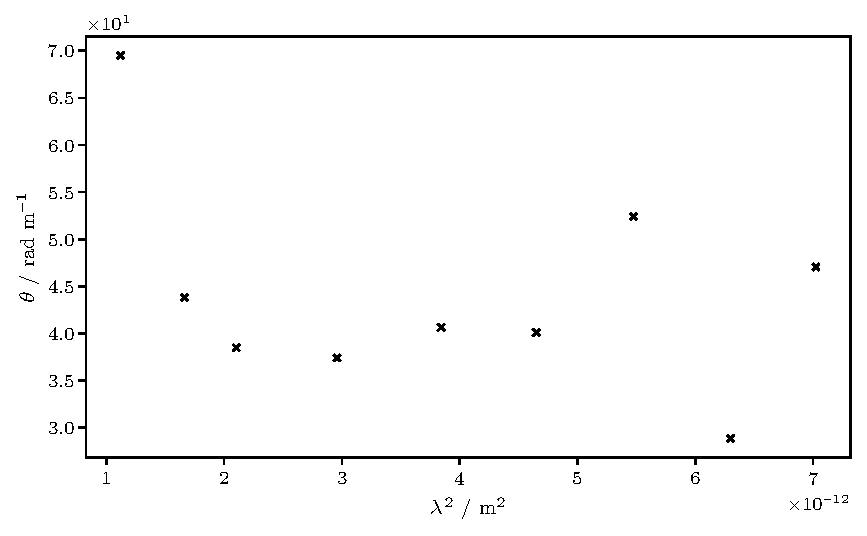
\includegraphics{build/doped-1.pdf}
    \caption{Messung zum normierten Drehwinkel für n-GaAs (1).}
    \label{fig:dotiert-1}
\end{figure}

Für n-GaAs (2) wurde ebenfalls die Differenz der Messwerte normiert auf eine Feldstärke von $B$ an Stelle von $2 \cdot B$.
Dies wurde äquivalent wie in dem Plot \ref{fig:dotiert-1} in dem Plot \ref{fig:dotiert-2} aufgetragen.

\begin{figure}[H]
    \centering
    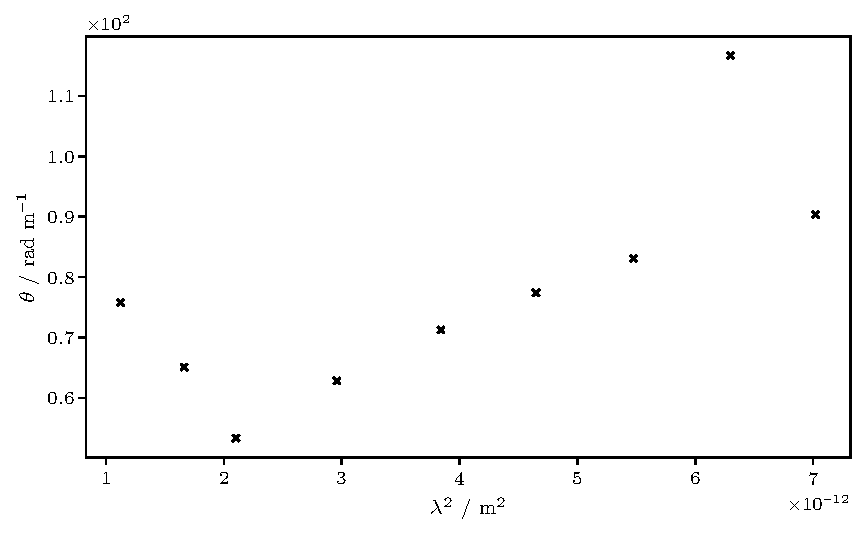
\includegraphics{build/doped-2.pdf}
    \caption{Messung zum normierten Drehwinkel für n-GaAs (2).}
    \label{fig:dotiert-2}
\end{figure}

\subsubsection{Reine Probe}

Die hochreine GaAs Probe hat eine Dicke von $L = \qty{5.11}{\milli\meter}$.
Für die Messwerte der reinen GaAs Probe wurde wie in dem Abschnitt \ref{sec:Dotierte} verfahren.
Anschließend wurden die Winkel-Werte gegenüber der Wellenlänge der Interferenzfilter zum Quadrat in dem Plot \ref{fig:rein}
aufgetragen.

\begin{figure}[H] 
    \centering
    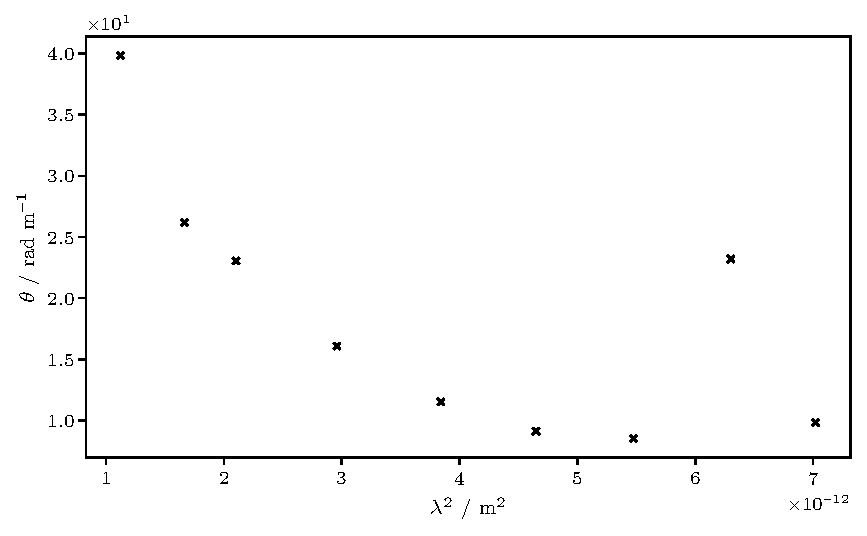
\includegraphics{build/pure.pdf}
    \caption{Messung zum normierten Drehwinkel für GaAs.}
    \label{fig:rein}
\end{figure}

\subsection{Effektive Masse}

$n = \num{3.397}$ \cite{brechungsindex}

$c = \input{build/c.tex}$

$e_0 = \input{build/e-0.tex}$

$m_0 = \input{build/m-0.tex}$

$m^{*} = (\num{0.078(0.004)})\,m_0$ \cite{PhysRev.114.59}

\begin{align*}
    \pfrac{\theta}{L} = a \lambda^2 + b
\end{align*}

\eqref{eqn:ausgleichsrechnung}

\begin{align*}
    m^* = \sqrt{\pfrac{Ne_0^3B}{8\pi^2 \varepsilon_0 c^3 n a}}
\end{align*}

\begin{align*}
    a = \input{build/a-1.tex} && b = \input{build/b-1.tex}
\end{align*}

$m^{*}_1 = \input{build/m-1.tex}$

\begin{align*}
    a = \input{build/a-2.tex} && b = \input{build/b-2.tex}
\end{align*}

$m^{*}_2 = \input{build/m-2.tex}$

\begin{figure}[H]
    \centering
    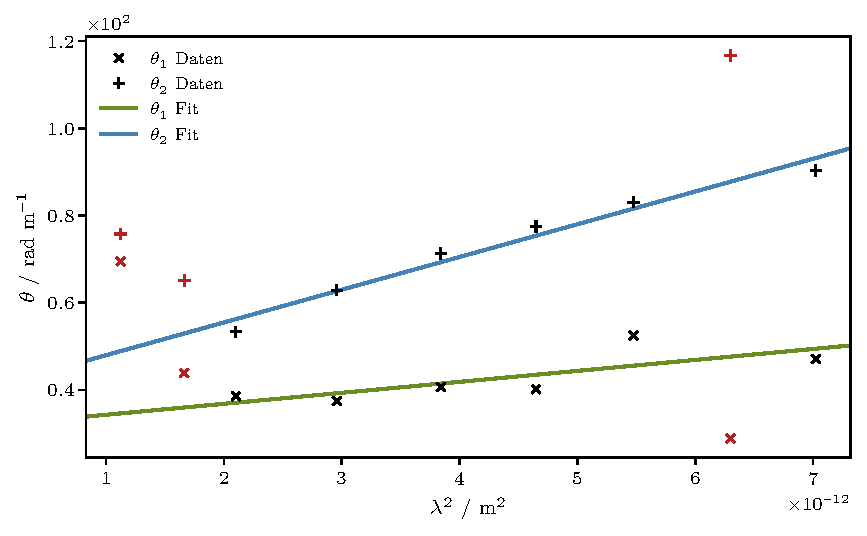
\includegraphics{build/mass.pdf}
    \caption{Ergebnisse und Ausgleichgeraden zum Drehwinkel aus Wirkung der Leitungselektronen.
             Hervorgehobene Datenpunkte werden ausgelassen.}
    \label{fig:masse}
\end{figure}
